%!TEX root = ../main.tex

\chapter{总结和展望}

\section{相关工作总结}

本模板主要内容来源于ZJU-Awesome项目,
参考软件学院论文格式要求做出调整,
并加入补充宏包,调整若干属性配置完成。
封面方面主要调整了各栏间距和对齐,
摘要依照软件学院更改了关键字的样式和页码的样式。
软件学院规定从摘要起每页必须有对应章标题的页眉,
虽然在一般排版习惯里,章头处不应设置页眉,
但考虑到已有大部分同学使用Word字处理软件遵照执行,
为保一致性,本模板暂时向软件学院的设定妥协。
由于论文格式要求并未向章头处的间距做出任何设定,
本模板保留ZJU-Awesome设定。
除此之外,本模板还做出了不少微小的改动。
详情请仔细阅读\texttt{zjuthesis.cls}和\texttt{main.tex}相关内容。

考虑到大部分软件学院的同学对\LaTeX 论文排版的陌生,
本文以尽量精炼的篇幅介绍了论文排版工作的各方面。
现在给出一个参考流程如\autoref{fig:workflow} 希望能对初次使用
\LaTeX 排版论文的同学一点提示。

\begin{figure}[htbp]
    \centering
    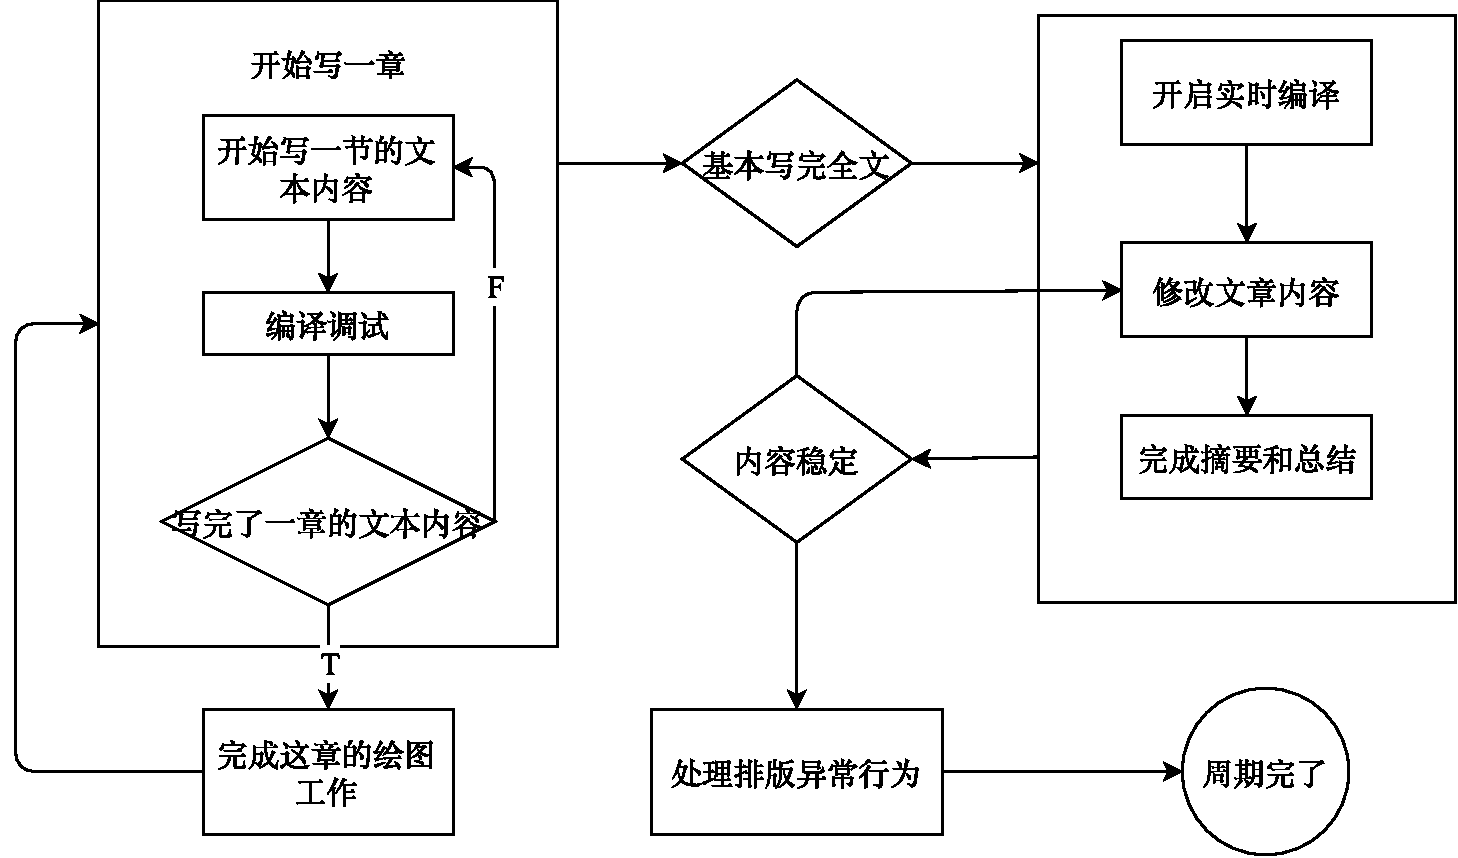
\includegraphics[width=.8\textwidth]{workflow.pdf}
    \caption{论文排版工作参考流程}
    \label{fig:workflow}
\end{figure}

\section{研究工作展望}

本文没有讨论各式\LaTeX 环境的使用细则,宏包的具体细节,
调试查错的技巧,也几乎没有交待任何一种具体的绘图方案。
希望屏幕前的你能以最少的代价完成论文排版工作,
养成内容和样式分离的电子写作习惯,
并能独立思考信息表达的最佳模式。

本文草拟于2016年夏季毕业论文送审前,
希望本文能抛砖引玉,
对\LaTeX 有经验的后辈们若能继续完善甚至颠覆本模板的设定,
相信一定能对软件学院的论文排版素质起到根本的改善作用。
